\chapter{节拍脉冲发生器时序电路实验}

\section{实验内容}

本实验分为三个子实验:

\begin{itemize}
    \item 连续节拍发生电路设计
    \item 单步节拍发生电路设计
    \item 单步/连续节拍发生电路设计
\end{itemize}

要求先单独设计出连续、单步节拍发生电路,然后将它们组合到一个电路里,并设计控制切换的电路。

\section{实验原理}

\subsection{连续节拍发生电路}

\begin{figure}[h]
\centering
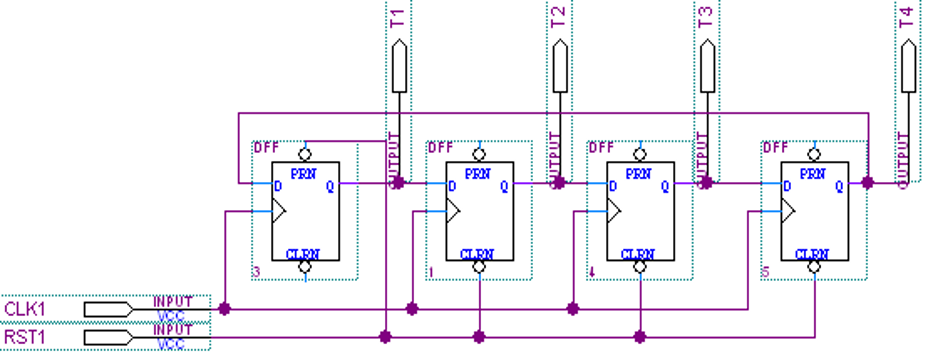
\includegraphics[width=\textwidth]{images/prin1_1.png}
\caption{连续节拍发生电路}
\label{fig:prin1_1}
\end{figure}

如图\ref{fig:prin1_1},由四个 D 触发器组成,可产生四个等间隔的时序信号 T1, T2, T3, T4。

\subsubsection{输入信号}

\begin{itemize}
    \item CLK1
    
    时钟信号。稳定的等间隔方波信号。
    
    \item RST1
    
    重置信号,连续节拍发生器的开关。
    
    可由外部控制的输入信号。
    
\end{itemize} 

\subsubsection{输出信号}

\begin{itemize}
    \item T1
    
    第一个输出信号。
    
    \item T2
    
    第二个输出信号。

    \item T3

    第三个输出信号。

    \item T4
    
    第四个输出信号。

\end{itemize}

\subsubsection{详细说明}

\begin{enumerate}
    \item RST1 = 0
    
    第一个 D 触发器的 PRN = 0 (低有效),强制 Q = 1 因此 T1 = 1;
    
    其他 D 触发器的 CLRN = 0 (低有效),强制 Q = 0 因此 T2 = T3 = T4 = 1。
    
    \item RST1 = 1
    
    这个时候实际上 RST1 对电路是没有其他影响的,触发器的 PRN, CLRN 都处于无效态。
    
    对于任意一个 D 触发器,将在下一个 CLK1 上升沿使得 Q := D。由于四个 D 触发器的 Q, D 首尾相连,实际上它们在每个 CLK1 上升沿时,将前一个 D 触发器的输出电位“搬运”到下一个 D 触发器输出电位。周而复始,形成连续节拍发生器。
    
    其周期为 CLK1 周期的4倍。
    
\end{enumerate}

\subsection{单步节拍发生电路}

\begin{figure}[h]
\centering
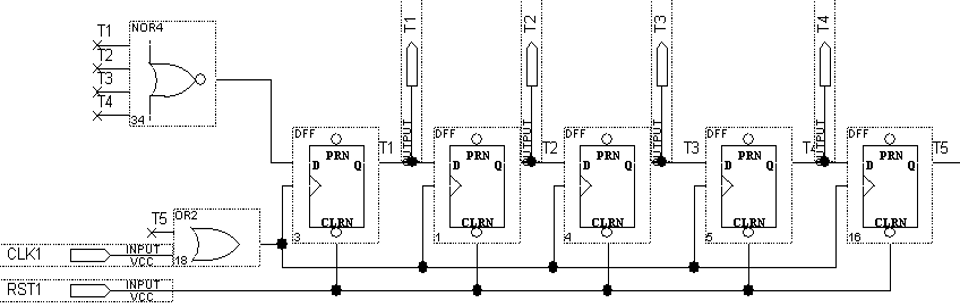
\includegraphics[width=\textwidth]{images/prin1_2.png}
\caption{单步节拍发生电路}
\label{fig:prin1_2}
\end{figure}

如图\ref{fig:prin1_2},由五个 D 触发器、一个 4 路或非门、一个 2 路或门组成,可产生四个等间隔的时序信号 T1, T2, T3, T4。

\subsubsection{输入信号}

\begin{itemize}
    \item CLK1
    
    时钟信号。稳定的等间隔方波信号。
    
    \item RST1
    
    重置信号,每个上升产生一个单步信号。
    
    是可由外部控制的输入信号。
    
\end{itemize} 

\subsubsection{输出信号}

\begin{itemize}
    \item T1
    
    第一个输出信号。
    
    \item T2
    
    第二个输出信号。

    \item T3

    第三个输出信号。

    \item T4
    
    第四个输出信号。

\end{itemize}

\subsubsection{详细说明}

\begin{enumerate}
    \item RST1 = 0
    
    所有 D 触发器 CLRN = 0 (低有效),T1 = T2 = T3 = T4 = T5 = Q = 0。
    
    注意此时第一个 D 触发器的输入是 D = NOR(T1, T2, T3, T4) = NOR(0, 0, 0, 0) = 1,这相当于一个单步时序的初始化。
    
    T5 = 0 使得 OR(CLK1, T5) = CLK1,此时 2 路或门没有作用。
    
    \item RST1 = 1
    
    所有 D 触发器的 PRN, CLRN 都处于无效态。
    
    在 RST1 = 1 后的第一个 CLK1 上升沿,第一个 D 触发器的 T1 = Q := D = 1,T1 = 1 时 4 路或非门将输出 0,因此第一个 D 触发器的 D端将马上被置为 0,这样就能保证只产生一个信号。
    
    在第二、三、四个 CLK1 上升沿,同连续时序发生器,电位在触发器之间被“搬运”,T2, T3, T4 相继输出1,然后复位。
    
    在第五个 CLK1 上升沿,T5 := 1,2 路或门的输出保持为1,屏蔽时钟信号对节拍发生器的影响。
        
\end{enumerate}

\subsection{单步/连续节拍发生电路}


\begin{figure}[h]
\centering
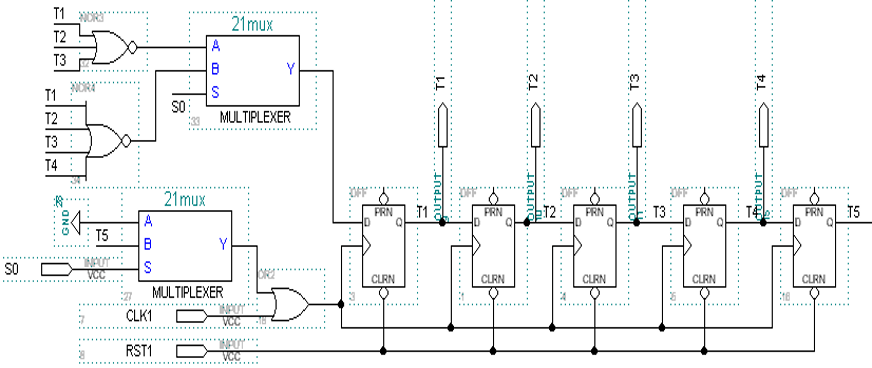
\includegraphics[width=\textwidth]{images/prin1_3.png}
\caption{单步/连续节拍发生电路}
\label{fig:prin1_3}
\end{figure}

如图\ref{fig:prin1_3},由五个 D 触发器、一个 4 路或非门、一个 3 路或非门、一个 2 路或门、两个 2 选 1 选择器组成,可产生四个等间隔的时序信号 T1, T2, T3, T4。

\subsubsection{输入信号}

\begin{itemize}
    \item CLK1
    
    时钟信号。稳定的等间隔方波信号。
    
    \item RST1
    
    重置信号,每个上升产生一个单步信号。
    
    是可由外部控制的输入信号。
    
    \item S0
    
    选择信号,0:单步;1:连续。
    
    是可由外部控制的输入信号。
    
\end{itemize} 

\subsubsection{输出信号}

\begin{itemize}
    \item T1
    
    第一个输出信号。
    
    \item T2
    
    第二个输出信号。

    \item T3

    第三个输出信号。

    \item T4
    
    第四个输出信号。

\end{itemize}

\subsubsection{详细说明}

\begin{enumerate}
    \item S0 = 0
    
    选择器 B 端导通,图 \ref{fig:prin1_3} 可化简为 图 \ref{fig:prin1_2},即单步时序发生器。
    
    \item S0 = 1
    
    选择器 A 端导通,图 \ref{fig:prin1_3} 可化简:
    
    \begin{itemize}
        \item 2 路或门的一个输入接地,相当于或门无作用,可消去。
        \item T5 断路,连带第五个 D 触发器的输出断路,因此该触发器无效,可消去。
    \end{itemize}
    
    此时类似单步时序发生器的原理,在 RST1 = 0 时由 3 路或非门给出第一个高电平信号;在 RST1 = 1 时“搬运”该信号,当 T4 = 1 时,可知 T1 = T2 = T3 = 0, 3 路或非门又将产生一个新的高电平信号。周而复始,构成连续时序发生器。
        
\end{enumerate}

\section{实验任务}

\subsection{连续节拍发生电路设计}

\subsection{单步节拍发生电路设计}

\subsubsection{没有 T5 输入下的仿真波形图}

\begin{figure}[h]
\centering
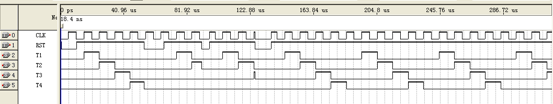
\includegraphics[width=\textwidth]{images/wave1_2_1.png}
\caption{没有 T5 输入时的仿真波形图}
\label{fig:wave1_2_1}
\end{figure}

若 2 路或门没有 T5 输入而是 GND 输入,或门失效,可消去。

当高电位“搬运”至 T5 时,T1 = T2 = T3 = T4 = 0, 4 路或非门将输出 1,产生新的高电平。

这样就化为连续节拍发生器了。

由此说明,T5 输入的作用在于屏蔽时钟信号,阻止下一节拍的发生。

由此引发思考:如果直接在单步节拍发生电路的基础上,将 T5 输入改为 AND(NOT(S0), T5),就产生了单步/连续节拍发生器。

这与原理图 \ref{fig:prin1_3} 的区别在于连续时序发生器的周期不同,在高电位搬运至 T5 时没有输出 T5,相当于产生了一个空节拍。

重新思考原理图 \ref{fig:prin1_3} 还是能发现一些冗余、可以优化的地方,例如 3 路或非门可以通过将“先选择,后或非”的方式合并到 4 路或非门中。

\subsection{单步/连续节拍发生电路设计}

\subsection{思考题}

\begin{enumerate}
    \item 单步运行与连续运行有何区别,它们各自的使用环境怎样?
    
    \item 如何实现单步/连续运行工作方式的切换?
    
\end{enumerate}

\section{实验步骤}
